\ifdefined\ispartofbook
\else
  % Preamble for "A Journey into Deep Learning"

% --- DOCUMENT CLASS & GEOMETRY ---
\documentclass[11pt, a4paper]{report} % Changed from 'article' to 'report' to enable \chapter command
\usepackage[margin=1in]{geometry} % Set page margins

% --- FONT & ENCODING ---
\usepackage[T1]{fontenc}
\usepackage[utf8]{inputenc}

% --- MATHEMATICS & SYMBOLS ---
\usepackage{amsmath, amssymb, amsthm} % For advanced math typesetting and theorems
\usepackage{amsfonts}                 % For math fonts
\usepackage{bm}                       % For bold math symbols

% --- GRAPHICS & TABLES ---
\usepackage{graphicx}                 % To include graphics
\usepackage{booktabs}                 % For professional-quality tables
\usepackage{caption}                  % For customizing captions

% --- LISTS & LAYOUT ---
\usepackage{enumitem}                 % For list customization
\usepackage{cases}                    % For cases environment

% --- TIKZ GRAPHICS PACKAGES (NEWLY ADDED) ---
\usepackage{tikz}
\usetikzlibrary{
    positioning,
    arrows.meta,
    fit,
    decorations.pathreplacing,
    calligraphy,
    shapes.geometric,
    shadows,
    chains,
    backgrounds % For layering
}

% --- HYPERLINKS & URLS ---
\usepackage[hyphens]{url}             % For URL formatting
\usepackage{hyperref}                 % For hyperlinks and cross-references
\hypersetup{
    colorlinks=true,
    linkcolor=blue,
    filecolor=magenta,
    urlcolor=cyan,
    citecolor=red,
}

% --- CUSTOM COMMANDS ---
\newcommand{\vect}[1]{\mathbf{#1}}
\newcommand{\matr}[1]{\mathbf{#1}}
\newcommand{\normdist}{\mathcal{N}}
\newcommand{\reals}{\mathbb{R}}
\newcommand{\E}{\mathbb{E}}

  \begin{document}
\fi

\chapter{The Rectified Linear Unit: Deep Learning's Dominant Non-Linearity}
\label{chap:relu}

% This file defines the command for plotting the ReLU function.
% It can be compiled standalone or included in a larger document.

\ifdefined\ispartofbook
\else
  % --- Standalone Compilation Preamble ---
  \documentclass[tikz, border=10pt]{standalone}
  \usepackage{tikz}
  \usetikzlibrary{arrows.meta}
  \begin{document}
\fi

% --- THE DIAGRAM COMMAND ---
\newcommand{\reluplot}{%
    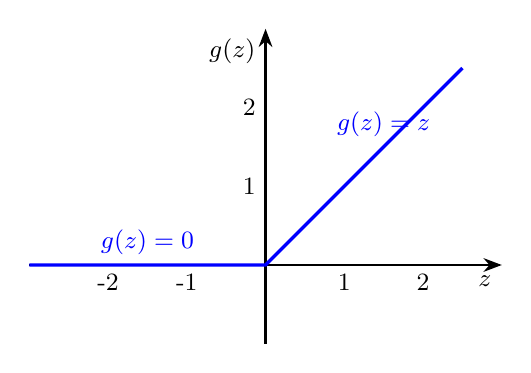
\begin{tikzpicture}[
        font=\sffamily,
        every node/.style={font=\small}
    ]
    % Axes
    \draw[-Stealth, thick] (-3,0) -- (3,0) node[below left] {$z$};
    \draw[-Stealth, thick] (0,-1) -- (0,3) node[below left] {$g(z)$};

    % Axis labels
    \node[below] at (-2, 0) {-2};
    \node[below] at (-1, 0) {-1};
    \node[below] at (1, 0) {1};
    \node[below] at (2, 0) {2};
    \node[left] at (0, 1) {1};
    \node[left] at (0, 2) {2};

    % ReLU function plot
    \draw[blue, very thick] (-3,0) -- (0,0) -- (2.5,2.5);

    % Annotations
    \node[above, blue] at (1.5, 1.5) {$g(z)=z$};
    \node[above, blue] at (-1.5, 0) {$g(z)=0$};
    
    \end{tikzpicture}%
}

\ifdefined\ispartofbook
  % This part is intentionally left blank when included in the main book.
  % The \newcommand is defined, and the chapter file is responsible for calling it.
\else
  % This part is for standalone compilation of the image.
  \reluplot
  \end{document}
\fi
 % Include the ReLU plot command file
% This file defines the command for plotting the Softplus and ReLU functions.
% It can be compiled standalone or included in a larger document.

\ifdefined\ispartofbook
\else
  % --- Standalone Compilation Preamble ---
  \documentclass[tikz, border=10pt]{standalone}
  \usepackage{tikz}
  \usetikzlibrary{arrows.meta}
  \begin{document}
\fi

% --- THE DIAGRAM COMMAND ---
\newcommand{\softplusplot}{%
    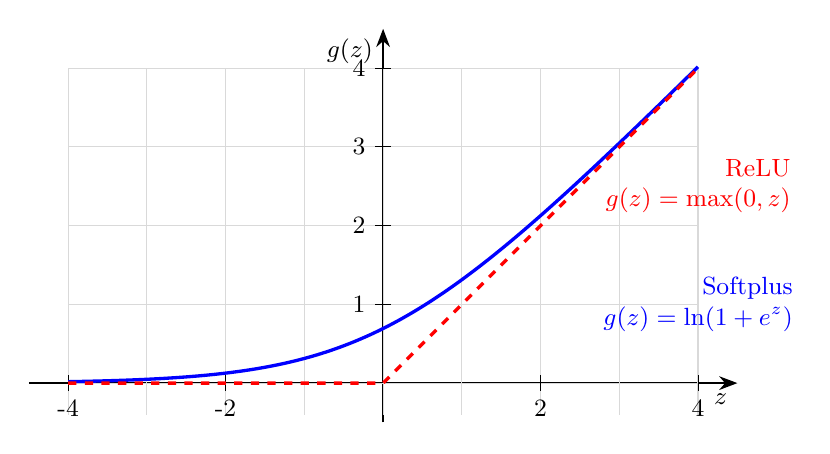
\begin{tikzpicture}[
        font=\sffamily,
        every node/.style={font=\small}
    ]
    % Axes
    \draw[-Stealth, thick] (-4.5,0) -- (4.5,0) node[below left] {$z$};
    \draw[-Stealth, thick] (0,-0.5) -- (0,4.5) node[below left] {$g(z)$};

    % Grid
    \draw[gray!30, thin, step=1] (-4,-0.4) grid (4,4);

    % Axis labels
    \foreach \x in {-4, -2, 2, 4}
        \draw (\x, 0.1) -- (\x, -0.1) node[below] {\x};
    \foreach \y in {1, 2, 3, 4}
        \draw (0.1, \y) -- (-0.1, \y) node[left] {\y};

    % Softplus function plot
    \draw[blue, very thick, smooth, domain=-4:4, samples=100] plot (\x, {ln(1+exp(\x))});

    % ReLU function plot for comparison
    \draw[red, very thick, dashed] (-4,0) -- (0,0) -- (4,4);
    
    % Legend
    \node[blue, align=right] at (4,1) {Softplus \\ $g(z)=\ln(1+e^z)$};
    \node[red, align=right] at (4,2.5) {ReLU \\ $g(z)=\max(0,z)$};
    
    \end{tikzpicture}%
}

\ifdefined\ispartofbook
  % This part is intentionally left blank when included in the main book.
  % The \newcommand is defined, and the chapter file is responsible for calling it.
\else
  % This part is for standalone compilation of the image.
  \softplusplot
  \end{document}
\fi
 % Include the Softplus plot command file
% This file defines the command for plotting the Sigmoid and Tanh functions.
% It can be compiled standalone or included in a larger document.

\ifdefined\ispartofbook
\else
  % --- Standalone Compilation Preamble ---
  \documentclass[tikz, border=10pt]{standalone}
  \usepackage{tikz}
  \usetikzlibrary{arrows.meta}
  \begin{document}
\fi

% --- THE DIAGRAM COMMAND ---
\newcommand{\saturatingplot}{%
    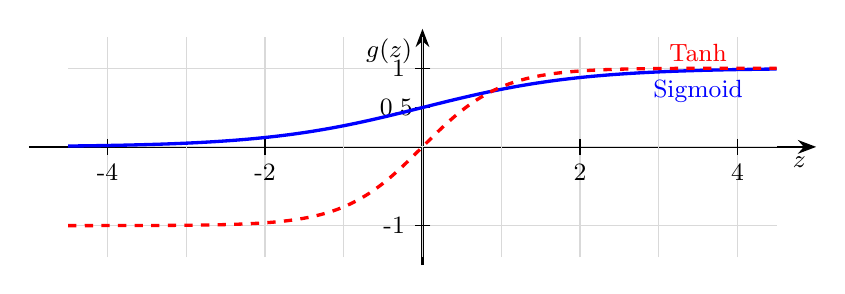
\begin{tikzpicture}[
        font=\sffamily,
        every node/.style={font=\small}
    ]
    % Axes
    \draw[-Stealth, thick] (-5,0) -- (5,0) node[below left] {$z$};
    \draw[-Stealth, thick] (0,-1.5) -- (0,1.5) node[below left] {$g(z)$};

    % Grid
    \draw[gray!30, thin, step=1] (-4.5,-1.4) grid (4.5,1.4);

    % Axis labels
    \foreach \x in {-4, -2, 2, 4}
        \draw (\x, 0.1) -- (\x, -0.1) node[below] {\x};
    \foreach \y in {-1, 1}
        \draw (0.1, \y) -- (-0.1, \y) node[left] {\y};
    \node[left] at (0, 0.5) {0.5};
    \draw (0.1, 0.5) -- (-0.1, 0.5);


    % Sigmoid function plot
    \draw[blue, very thick, smooth, domain=-4.5:4.5, samples=100] plot (\x, {1/(1+exp(-\x))});

    % Tanh function plot
    \draw[red, very thick, dashed, smooth, domain=-4.5:4.5, samples=100] plot (\x, {tanh(\x)});
    
    % Legend
    \node[blue] at (3.5, 0.7) {Sigmoid};
    \node[red] at (3.5, 1.2) {Tanh};
    
    \end{tikzpicture}%
}

\ifdefined\ispartofbook
  % This part is intentionally left blank when included in the main book.
  % The \newcommand is defined, and the chapter file is responsible for calling it.
\else
  % This part is for standalone compilation of the image.
  \saturatingplot
  \end{document}
\fi
 % Include the Sigmoid/Tanh plot command file
% This file defines the command for plotting the standard normal PDF and CDF.
% It can be compiled standalone or included in a larger document.

\ifdefined\ispartofbook
\else
  % --- Standalone Compilation Preamble ---
  \documentclass[tikz, border=10pt]{standalone}
  \usepackage{tikz}
  \usetikzlibrary{arrows.meta}
  % No longer need pgfplots, as we are using pre-computed coordinates
  \begin{document}
\fi

% --- THE DIAGRAM COMMAND ---
\newcommand{\normalpdfcdfplot}{%
    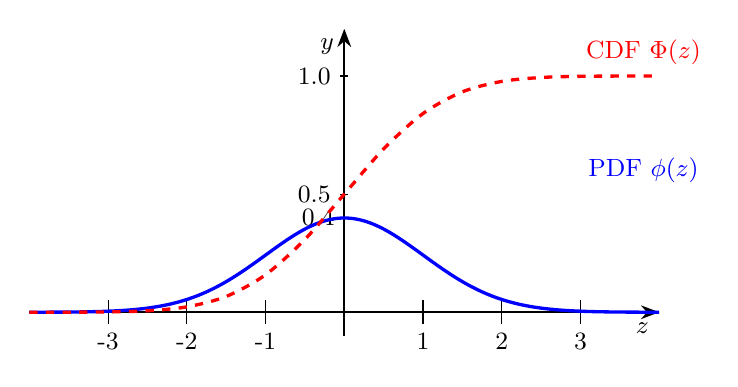
\begin{tikzpicture}[
        x=1cm, y=3cm, % Set vertical unit larger than horizontal to make plot taller
        font=\sffamily,
        every node/.style={font=\small}
    ]
    % Axes
    \draw[-Stealth, thick] (-4,0) -- (4,0) node[below left] {$z$};
    \draw[-Stealth, thick] (0,-0.1) -- (0,1.2) node[below left] {$y$};

    % Axis labels
    \foreach \x in {-3, -2, -1, 1, 2, 3}
        \draw (\x, 0.05) -- (\x, -0.05) node[below] {\x};
    \foreach \y/\ytext in {0.5/{0.5}, 1/{1.0}}
        \draw (0.05, \y) -- (-0.05, \y) node[left] {\ytext};
    \node[left] at (0, 0.4) {0.4}; % For PDF peak

    % PDF plot (bell curve) using the built-in gaussian function
    \draw[blue, very thick, smooth, domain=-4:4, samples=100] plot (\x, {1/sqrt(2*pi)*exp(-(\x*\x)/2)});

    % CDF plot (S-shaped curve) using pre-computed coordinates to avoid 'erf' dependency
    \draw[red, very thick, dashed, smooth] plot coordinates {
        (-4.0, 0.00003) (-3.5, 0.0002) (-3.0, 0.0013) (-2.5, 0.0062) 
        (-2.0, 0.0228) (-1.5, 0.0668) (-1.0, 0.1587) (-0.5, 0.3085) 
        (0.0, 0.5) (0.5, 0.6915) (1.0, 0.8413) (1.5, 0.9332) 
        (2.0, 0.9772) (2.5, 0.9938) (3.0, 0.9987) (3.5, 0.9998) 
        (4.0, 0.99997)
    };
    
    % Legend
    \node[blue, align=right] at (3.8, 0.6) {PDF $\phi(z)$};
    \node[red, align=right] at (3.8, 1.1) {CDF $\Phi(z)$};
    
    \end{tikzpicture}%
}

\ifdefined\ispartofbook
  % This part is intentionally left blank when included in the main book.
  % The \newcommand is defined, and the chapter file is responsible for calling it.
\else
  % This part is for standalone compilation of the image.
  \normalpdfcdfplot
  \end{document}
\fi
 % Include the Normal PDF/CDF plot command file
% This file defines the command for the rectified moment calculation diagram.
% It can be compiled standalone or included in a larger document.

\ifdefined\ispartofbook
\else
  % --- Standalone Compilation Preamble ---
  \documentclass[tikz, border=10pt]{standalone}
  \usepackage{amsmath, amssymb} % For math symbols
  \usepackage{tikz}
  \usetikzlibrary{
    positioning,
    arrows.meta,
    shapes.geometric,
    chains
  }
  \begin{document}
\fi

% --- THE DIAGRAM COMMAND ---
\newcommand{\momentcalculationdiagram}{%
    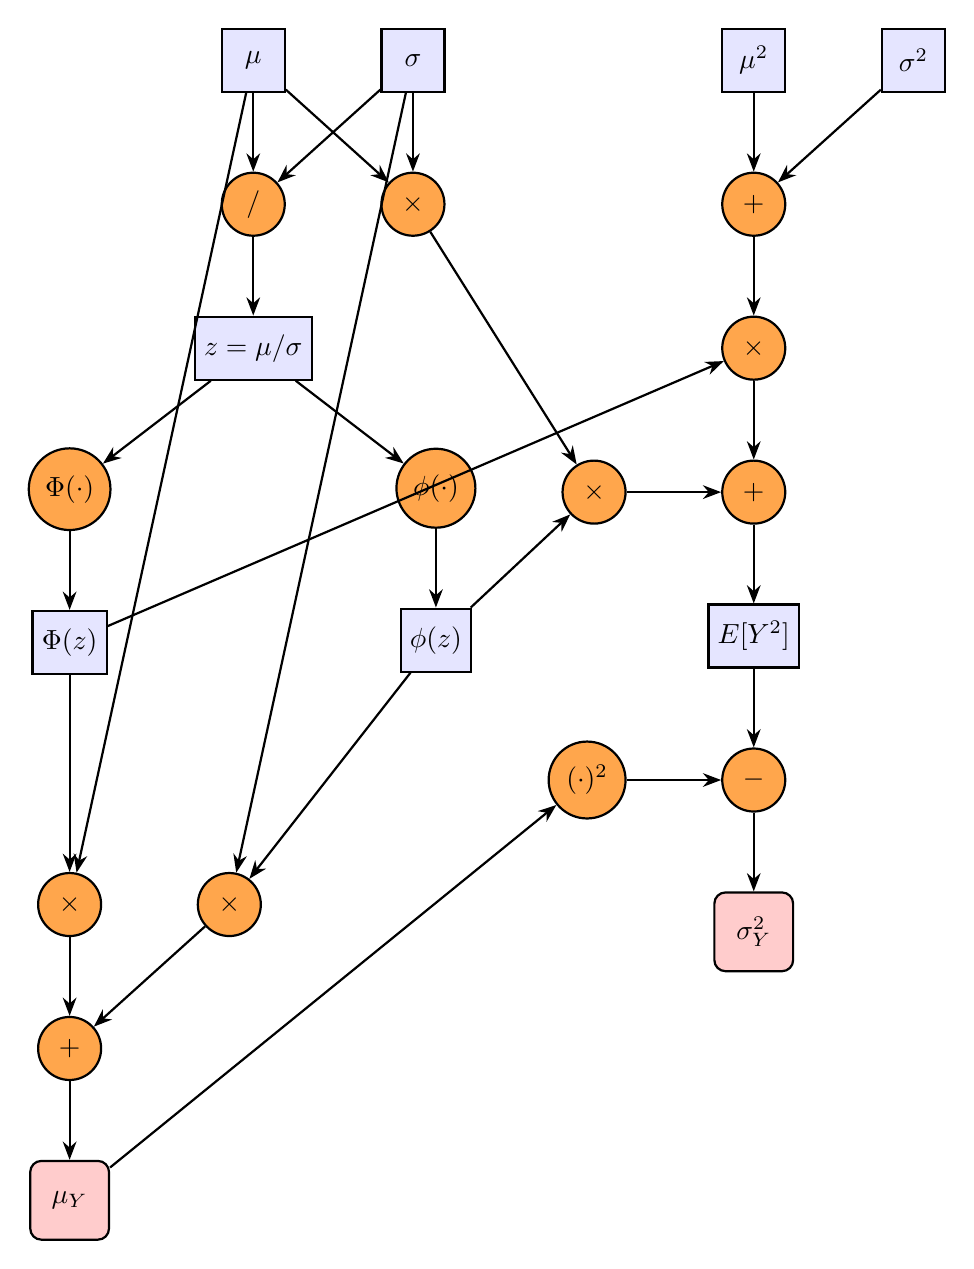
\begin{tikzpicture}[
        node distance=1cm and 1.2cm,
        data/.style={rectangle, draw, thick, minimum size=0.8cm, fill=blue!10},
        op/.style={circle, draw, thick, minimum size=0.8cm, fill=orange!70},
        func/.style={ellipse, draw, thick, minimum size=0.8cm, fill=green!20},
        final/.style={rectangle, draw, thick, rounded corners, minimum size=1cm, fill=red!20, font=\bfseries},
        arrow/.style={-Stealth, thick}
    ]
    % --- Initial Inputs ---
    \node[data] (mu) {$\mu$};
    \node[data, right=of mu] (sigma) {$\sigma$};

    % --- Intermediate Calculation Block (MODIFIED) ---
    \node[op, below=of mu] (div1) {$/$};
    \node[data, below=of div1] (z) {$z = \mu/\sigma$};
    
    % --- MODIFIED: Separated function from data for CDF and PDF ---
    \node[op, below left=of z] (cdf_func) {$\Phi(\cdot)$};
    \node[data, below=of cdf_func] (cdf_val) {$\Phi(z)$};
    \node[op, below right=of z] (pdf_func) {$\phi(\cdot)$};
    \node[data, below=of pdf_func] (pdf_val) {$\phi(z)$};
    
    \node[op, right=of div1] (mult5) {$\times$};

    % --- Mean Calculation Path ---
    \node[op, below=2.5cm of cdf_val] (mult1) {$\times$};
    \node[op, below=of mult1] (add1) {$+$};
    \node[op, right=of mult1] (mult2) {$\times$};
    \node[final, below=of add1] (mu_y) {$\mu_Y$};

    % --- Variance Calculation Path ---
    \node[data, right=3.5cm of sigma] (mu2) {$\mu^2$};
    \node[data, right=of mu2] (sigma2) {$\sigma^2$};
    \node[op, below=of mu2] (add2) {$+$};
    \node[op, below=of add2] (mult3) {$\times$};
    \node[op, below=of mult3] (add3) {$+$};
    \node[op, left=of add3] (mult4) {$\times$};
    \node[data, below=of add3] (e_y2) {$E[Y^2]$};
    
    % --- Final Variance Calculation Nodes ---
    \node[op, below=of e_y2] (op_minus) {$-$};
    \node[op, left=of op_minus] (op_sq) {$(\cdot)^2$};
    \node[final, below=of op_minus] (sigma2_y) {$\sigma^2_Y$};

    % --- Arrows for Inputs (MODIFIED) ---
    \draw[arrow] (mu) -- (div1);
    \draw[arrow] (sigma) -- (div1);
    \draw[arrow] (div1) -- (z);
    
    % --- MODIFIED: Arrows for new function nodes ---
    \draw[arrow] (z) -- (cdf_func);
    \draw[arrow] (z) -- (pdf_func);
    \draw[arrow] (cdf_func) -- (cdf_val);
    \draw[arrow] (pdf_func) -- (pdf_val);

    % --- Arrows for Mean Calculation (MODIFIED) ---
    \draw[arrow] (mu) -- (mult1);
    \draw[arrow] (cdf_val) -- (mult1);
    \draw[arrow] (sigma) -- (mult2);
    \draw[arrow] (pdf_val) -- (mult2);
    \draw[arrow] (mult1) -- (add1);
    \draw[arrow] (mult2) -- (add1);
    \draw[arrow] (add1) -- (mu_y);

    % --- Arrows for Variance Calculation (MODIFIED) ---
    \draw[arrow] (mu2) -- (add2);
    \draw[arrow] (sigma2) -- (add2);
    \draw[arrow] (add2) -- (mult3);
    \draw[arrow] (cdf_val) -- (mult3);
    
    \draw[arrow] (mu) -- (mult5);
    \draw[arrow] (sigma) -- (mult5);
    \draw[arrow] (mult5) -- (mult4);
    \draw[arrow] (pdf_val) -- (mult4);
    
    \draw[arrow] (mult3) -- (add3);
    \draw[arrow] (mult4) -- (add3);
    \draw[arrow] (add3) -- (e_y2);

    % --- Arrows for Final Variance Calculation ---
    \draw[arrow] (e_y2) -- (op_minus);
    \draw[arrow] (mu_y) -- (op_sq);
    \draw[arrow] (op_sq) -- (op_minus);
    \draw[arrow] (op_minus) -- (sigma2_y);

    \end{tikzpicture}%
}

\ifdefined\ispartofbook
  % This part is intentionally left blank when included in the main book.
\else
  % This part is for standalone compilation of the image.
  \momentcalculationdiagram
  \end{document}
\fi
 % Include the Moment Calculation diagram

This chapter will serve as a comprehensive introduction to the single most important component of modern deep learning: the Rectified Linear Unit (ReLU). The narrative will trace its journey from a statistical curiosity to the undisputed workhorse of neural networks. We will deconstruct why this simple function is so effective, exploring its historical context, its statistical soul, its inherent failure modes, and how it compares to other non-linearities. This chapter will establish the foundational building block upon which all subsequent concepts in the book are built. The story of ReLU is not merely one of engineering convenience; it is a story of emergent properties, where a simple mathematical form serendipitously solved the most critical bottlenecks that hindered the progress of artificial intelligence for years.

\section{From Biology to Backpropagation: The Rise of ReLU}
\label{sec:rise_of_relu}

The Rectified Linear Unit, defined by the elegantly simple function $f(x) = \max(0, x)$, has become the de facto standard activation function for deep neural networks, playing a central and indispensable role in the successes of modern deep learning \cite{DansbeckerRELUKaggle}. Its widespread adoption is often attributed to its computational simplicity and its remarkable empirical effectiveness in mitigating the vanishing gradient problem that plagued earlier network architectures. However, a purely functional or heuristic understanding of ReLU belies its deep and consequential connections to fundamental principles of probability, statistics, and even computational neuroscience.

\begin{figure}[h!]
    \centering
    \scalebox{1.0}{\reluplot}
    \caption{The Rectified Linear Unit (ReLU) activation function, $g(z) = \max(0, z)$. It is zero for all negative inputs and linear for all positive inputs.}
    \label{fig:relu_plot}
\end{figure}

\subsection{Early Origins and Conceptualizations}
The mathematical abstraction of a rectified linear function has strong roots in computational neuroscience, where it serves as a simplified but powerful model for the firing rate of a biological neuron. The core idea, observed in biological systems, is that a neuron remains largely inactive (its firing rate is zero) until the total input stimulus it receives surpasses a certain activation threshold. Once this threshold is crossed, its firing rate increases in a manner that is approximately linear with the strength of the input stimulus \cite{Socci1998RectifiedGaussian}. This threshold-linear response is a fundamental principle of neural computation, providing a mechanism for selective information processing.

Early precursors to ReLU can be seen in several pioneering models that sought to emulate this biological behavior. In 1980, Kunihiko Fukushima's "Neocognitron," a groundbreaking hierarchical neural network designed for visual pattern recognition, used a form of rectification for visual feature extraction, laying some of the earliest groundwork for what would become modern convolutional networks \cite{Fukushima1980Neocognitron}. A decade later, in a different domain, Jerome Friedman's statistical method, Multivariate Adaptive Regression Splines (MARS), built predictive models from a basis of "hinge functions" of the form $\max(0, x-t)$ and $\max(0, t-x)$, which are clearly shifted and reflected versions of the ReLU function.

Despite these early appearances, the broader neural network community of the 1990s and early 2000s favored smooth, differentiable activation functions like the logistic sigmoid and the hyperbolic tangent (tanh). The prevailing wisdom was that the smoothness of these functions was essential for gradient-based optimization.

\begin{figure}[h!]
    \centering
    \scalebox{0.9}{\saturatingplot}
    \caption{The Sigmoid and hyperbolic tangent (Tanh) activation functions. Both are smooth and "saturate" at their minimum and maximum values, leading to vanishing gradients.}
    \label{fig:saturating_plot}
\end{figure}

\subsection{The Modern Ascent}
The modern history of ReLU began in earnest at the turn of the 21st century. The work of Hahnloser et al. (2000) is a crucial landmark, as it was the first to introduce the rectifier to a dynamical network with strong biological and mathematical justifications. The tipping point that ignited its widespread adoption in the deep learning community came with two key papers that addressed the most pressing challenges of the time.

First, Nair \& Hinton (2010) introduced ReLU to modern deep learning in the context of Restricted Boltzmann Machines (RBMs), a type of generative model used for the then-dominant paradigm of unsupervised pre-training. They argued that ReLU was a computationally efficient and highly effective approximation to the smoother Softplus function, $f(x) = \log(1+e^x)$, and demonstrated its superiority for feature learning tasks \cite{NairHinton2010ReLU}.

\begin{figure}[h!]
    \centering
    \scalebox{1.0}{\softplusplot}
    \caption{A comparison of the ReLU function (dashed red) and the Softplus function (solid blue). Softplus is a smooth, differentiable approximation of ReLU.}
    \label{fig:softplus_plot}
\end{figure}

Second, and perhaps most influentially, Glorot, Bordes, \& Bengio (2011) cemented its status by conducting a systematic analysis showing that deep \textit{supervised} networks using ReLU could achieve state-of-the-art performance \textit{without} the cumbersome, layer-by-layer unsupervised pre-training that was previously thought necessary \cite{GlorotBordesBengio2011DeepSparse}. They were the first to clearly articulate and empirically validate the key advantages of ReLU over the saturating functions that were dominant at the time.

\subsection{The Three Pillars of ReLU's Success}
The superiority of ReLU over its predecessors stems from three core advantages that directly address the primary challenges of training deep neural networks.

\begin{enumerate}
    \item \textbf{Computational Efficiency:} The ReLU function is computationally trivial. It requires only a single comparison and potentially a single assignment. This is a stark contrast to the expensive exponentiations required to compute sigmoid ($\sigma(x) = 1 / (1+e^{-x})$) and tanh functions. In deep networks with millions or even billions of parameters, this difference in computational cost per neuron translates into significantly faster training and inference times. This efficiency is not a minor convenience; it is a critical enabler for iterating on and deploying the massive models that define the state-of-the-art.

    \item \textbf{Alleviation of the Vanishing Gradient Problem:} For any positive input, the derivative of ReLU is a constant 1. This is fundamentally different from sigmoid and tanh, whose gradients are $\sigma'(x) = \sigma(x)(1-\sigma(x))$ and $\tanh'(x) = 1 - \tanh^2(x)$, respectively. These gradients are maximal at $x=0$ but approach zero as the input magnitude increases (i.e., as the neuron saturates). In a deep network, the gradient at a lower layer is the product of the gradients of all subsequent layers. With sigmoid or tanh units, this product involves multiplying many numbers less than 1, causing the gradient to shrink exponentially as it propagates backward. This is the famous "vanishing gradient problem," which makes it nearly impossible for lower layers to learn meaningful features. ReLU's constant gradient of 1 for active neurons breaks this destructive chain of multiplication, allowing error signals to reach deep into the network and enabling the effective training of much deeper architectures than was previously possible.

    \item \textbf{Induction of Sparse Activations:} ReLU outputs a true zero for any negative input. In a randomly initialized network, this means that for any given input sample, roughly 50\% of the hidden units will be inactive (outputting zero). This phenomenon, known as sparse activation, confers several benefits. A sparse representation is less entangled and more robust to small input perturbations. From a biological perspective, it is metabolically efficient. Computationally, it can be exploited by hardware and software to accelerate computation, as operations involving zero-valued activations can be skipped \cite{GlorotBordesBengio2011DeepSparse}. This sparsity acts as a natural form of regularization, reducing the co-adaptation of neurons and often leading to better generalization.
\end{enumerate}

\begin{table}[h!]
\centering
\caption{Comparison of common activation functions.}
\label{tab:activation_comparison}
\begin{tabular}{@{}llll@{}}
\toprule
\textbf{Function} & \textbf{Formula} & \textbf{Output Range} & \textbf{Key Pathologies} \\ \midrule
Sigmoid & $\frac{1}{1+e^{-x}}$ & $(0, 1)$ & Vanishing gradient, Not zero-centered \\
Tanh & $\frac{e^x - e^{-x}}{e^x + e^{-x}}$ & $(-1, 1)$ & Vanishing gradient \\
ReLU & $\max(0, x)$ & $[0, \infty)$ & Dying ReLU, Not zero-centered \\ \bottomrule
\end{tabular}
\end{table}

\section{The Statistical Soul of ReLU: Truncated and Rectified Distributions}
\label{sec:statistical_soul}

To fully comprehend the behavior of the Rectified Linear Unit, it is essential to first understand its statistical antecedents. The operation of rectification is not just an algorithmic choice; it is a well-defined statistical transformation. When a Gaussian-distributed random variable $X \sim \mathcal{N}(\mu, \sigma^2)$ is passed through a ReLU, the resulting distribution is known as a \textbf{rectified Gaussian distribution} \cite{Socci1998RectifiedGaussian}. This is a hybrid distribution, composed of two distinct parts:

\begin{enumerate}
    \item \textbf{A Discrete Mass at Zero:} All values of the original variable $X$ that were less than or equal to zero are mapped to the single output value $Y=0$. This creates a discrete probability mass, or "spike," at the origin. The magnitude of this mass is equal to the cumulative probability of the original Gaussian being non-positive. Let $\Phi(\cdot)$ be the cumulative distribution function (CDF) of the standard normal distribution $\mathcal{N}(0, 1)$. The probability of this discrete component is:
    \begin{equation}
    P(Y=0) = P(X \le 0) = P\left(\frac{X-\mu}{\sigma} \le \frac{-\mu}{\sigma}\right) = \Phi\left(-\frac{\mu}{\sigma}\right)
    \end{equation}

    \item \textbf{A Continuous Truncated Distribution:} For all values of $X$ that were positive, the rectification has no effect ($Y=X$). This portion of the probability mass remains distributed over the interval $(0, \infty)$. The resulting continuous component is a \textbf{truncated normal distribution}, which is the distribution of a normal random variable conditioned on it being greater than zero \cite{BarrSherrill1999TruncatedNormal}.
\end{enumerate}

The probability density function (PDF) of the rectified Gaussian variable $Y$ can be formally expressed using the Dirac delta function, $\delta(y)$, to represent the discrete mass at zero, and the Heaviside step function, $H(y)$, to represent the continuous part for $y > 0$:
\[ f_Y(y) = \Phi\left(-\frac{\mu}{\sigma}\right) \delta(y) + \frac{1}{\sigma} \phi\left(\frac{y-\mu}{\sigma}\right) H(y) \]
where $\phi(\cdot)$ and $\Phi(\cdot)$ are the standard normal PDF and CDF, respectively.

\begin{figure}[h!]
    \centering
    \scalebox{0.9}{\normalpdfcdfplot}
    \caption{The standard normal probability density function (PDF), $\phi(z)$, and cumulative distribution function (CDF), $\Phi(z)$. These functions are fundamental to the statistical analysis of rectified distributions.}
    \label{fig:normal_plot}
\end{figure}

This transformation fundamentally alters the moments of the distribution. The mean of the rectified variable, derived by integrating over the two parts of the distribution, is given by \cite{Socci1998RectifiedGaussian}:
\begin{equation}
 \mu_Y = \mu \Phi\left(\frac{\mu}{\sigma}\right) + \sigma \phi\left(\frac{\mu}{\sigma}\right)
\end{equation}
The variance is more complex but can also be derived analytically:
\begin{equation}
 \sigma^2_Y = (\mu^2 + \sigma^2)\Phi\left(\frac{\mu}{\sigma}\right) + \mu\sigma\phi\left(\frac{\mu}{\sigma}\right) - \mu_Y^2
\end{equation}

\begin{figure}[h!]
    \centering
    \scalebox{0.7}{\momentcalculationdiagram}
    \caption{A flowchart illustrating the calculation of the rectified mean ($\mu_Y$) and variance ($\sigma^2_Y$) from the original Gaussian parameters ($\mu, \sigma$).}
    \label{fig:moment_calculation}
\end{figure}

These formulas are the building blocks for Analytical Moment Propagation (AMP), a powerful framework for tracking the statistics of signals as they pass through a network \cite{Wright2024AnalyticCovariance}. The extension of these concepts to the multivariate case, where a vector of correlated Gaussian variables is rectified, forms the basis for the Rectified Multivariate Normal (RMVN) distribution, a powerful tool for modeling non-negative and sparse signals that will be explored in later chapters \cite{ChoSaul2014RectifiedGaussian}.

\section{Pathologies and Solutions: The "Dying ReLU" Problem}
\label{sec:dying_relu}

Despite its numerous advantages, the Rectified Linear Unit is not without its flaws. The most well-known and significant failure mode is the "dying ReLU" problem, a phenomenon where neurons can become permanently inactive during training, effectively reducing the capacity of the network and hindering the learning process.

This occurs when a large gradient update, often caused by an overly aggressive learning rate, pushes a neuron's weights and bias into a configuration where its pre-activation value, $z = \mathbf{w} \cdot \mathbf{x} + b$, is consistently negative for all data points in the training set. Once a neuron enters this state, it becomes trapped. Because the derivative of the ReLU function is zero for all negative inputs, the gradient flowing back to this neuron during backpropagation will always be zero. As a result, its weights and bias are never updated via gradient descent, and the neuron ceases to participate in the learning process. It becomes a dead end for information flow.

This has severe consequences for the network:
\begin{itemize}
    \item \textbf{Reduced Model Capacity:} Each dead neuron is effectively removed from the network's computational graph, reducing the number of active parameters and crippling its ability to learn complex functions.
    \item \textbf{Impaired Training:} The network is forced to rely on the remaining subset of active neurons to minimize the loss, which can lead to substantially increased training time or cause the optimization process to stagnate completely.
\end{itemize}

Fortunately, several effective techniques have been developed to mitigate this problem:
\begin{itemize}
    \item \textbf{Algorithmic Fixes:} The most direct solution is to use a lower learning rate, which reduces the magnitude of weight updates and makes it less likely that a single large gradient step will kill a neuron. Proper weight initialization is also critical. Using a scheme like He initialization ensures that neurons start in a healthy state, with pre-activations distributed around zero, reducing the likelihood of them dying early in training \cite{He2015Delving}.

    \item \textbf{Architectural Modifications:} The most common and robust solutions involve modifying the architecture of the activation function itself to eliminate the zero-gradient region. Several variants of ReLU have been proposed to mitigate this issue by introducing a small, non-zero slope for negative inputs. These include:
    \begin{itemize}
        \item \textbf{Leaky ReLU:} Defined as $f(x) = \max(\alpha x, x)$ for a small, fixed hyperparameter $\alpha$ (e.g., 0.01). The derivative for negative inputs is now $\alpha$, not 0. This ensures that the gradient never becomes truly zero, allowing a neuron that has been pushed into a negative regime to eventually recover and become active again.
        \item \textbf{Parametric ReLU (PReLU):} A generalization of Leaky ReLU where the leakage coefficient $\alpha$ is not a fixed hyperparameter but a learnable parameter that is updated via backpropagation along with the network's weights.
        \item \textbf{Exponential Linear Unit (ELU):} Uses an exponential function, $f(x) = \alpha(e^x - 1)$ for $x < 0$, which smoothly saturates to a negative value. This not only prevents dying neurons but can also push the mean activation of the layer closer to zero, which can accelerate learning.
    \end{itemize}
\end{itemize}
These solutions represent a fundamental trade-off. They prevent neuron death by ensuring a non-zero gradient everywhere, but in doing so, they necessarily sacrifice the property of true sparsity that the original ReLU provides. A Leaky ReLU neuron never outputs exactly zero (unless its input is exactly zero), meaning the representation is no longer truly sparse in the same way; it is merely "less active" in the negative regime.

\section{A Comparative Case Study: Why Not the Square Function?}
\label{sec:square_function_case_study}

To fully appreciate why ReLU is so effective, it is instructive to analyze a seemingly simple alternative: the quadratic function, $Y=X^2$. This function fails as a general-purpose activation for three fundamental reasons, highlighting the specific combination of properties that make ReLU successful.

\begin{enumerate}
    \item \textbf{Symmetric Information Loss:} The square function is an even function, satisfying the property $f(x) = f(-x)$. This means it irreversibly destroys the sign of the input. For any output $y > 0$, the input could have been either $\sqrt{y}$ or $-\sqrt{y}$. For example, inputs of -2 and +2 both map to an output of 4. This is a symmetric information loss, which is often more damaging than the asymmetric loss of ReLU, as it cannot distinguish between positive and negative signals of the same magnitude.

    \item \textbf{Unstable Gradient Dynamics:} The derivative, $f'(x) = 2x$, is unbounded and linearly dependent on the input's magnitude. This creates an untenable trade-off that makes robust training practically infeasible:
    \begin{itemize}
        \item For inputs with magnitude less than 0.5, the derivative's magnitude is less than 1. In a deep network, this leads to the product of many small numbers, causing gradients to shrink exponentially (the vanishing gradient problem).
        \item For inputs with magnitude greater than 0.5, the derivative's magnitude is greater than 1. This leads to the product of many large numbers, causing gradients to grow exponentially and training to diverge (the exploding gradient problem).
    \end{itemize}
    This inherent instability makes robust training of deep networks with square activations practically infeasible \cite{Hochreiter2001GradientFlow}.

    \item \textbf{Lack of Expressive Power:} A third, and perhaps most fatal, flaw lies in expressive power. A network composed of square activations can only represent polynomials of a certain degree. A key theorem in neural network theory, established by Pinkus (1999), proves that for a network to be a \textbf{universal approximator}—capable of approximating any continuous function to arbitrary precision—its activation function \textbf{cannot be a polynomial} \cite{Pinkus1999ApproximationTheory}. The activation must be non-polynomial to provide the necessary flexibility. In contrast, ReLU networks are universal approximators because they construct flexible, piecewise linear functions, which are not polynomials \cite{Hornik1989UniversalApprox}.
\end{enumerate}
This case study highlights that ReLU's success is not an accident but a result of a unique and robust balance of properties: a simple, non-saturating, and piecewise-linear nature that provides stable gradients and universal approximation capabilities. It is this combination that has made it the cornerstone of the deep learning revolution.

\ifdefined\ispartofbook
\else
  \begin{thebibliography}{99}

\bibitem{AdadiBerrada2018XAISurvey}
Adadi, A., \& Berrada, M. (2018). Peeking Inside the Black-Box: A Survey on Explainable Artificial Intelligence (XAI). \textit{IEEE Access}.

\bibitem{AlainBengio2016Probes}
Alain, G., \& Bengio, Y. (2016). Understanding intermediate layers using linear classifier probes. \textit{arXiv preprint arXiv:1610.01644}.

\bibitem{Amemiya1985Econometrics}
Amemiya, T. (1985). \textit{Advanced Econometrics}. Harvard University Press.

\bibitem{Arora2025ReLUOutputDist}
Arora, R., Basu, A., Mianjy, P., \& Mukherjee, A. (2025). On the Exact Computation of the Output Distribution of a ReLU Network. \textit{arXiv preprint arXiv:2503.22082}.

\bibitem{BarrSherrill1999TruncatedNormal}
Barr, D. R., \& Sherrill, E. T. (1999). Mean and variance of truncated normal distributions. \textit{The American Statistician, 53}(4), 357-361.

\bibitem{Bishop2006PatternRecognition}
Bishop, C. M. (2006). \textit{Pattern Recognition and Machine Learning}. Springer.

\bibitem{Bottou2018Optimization}
Bottou, L., Curtis, F. E., \& Nocedal, J. (2018). Optimization methods for large-scale machine learning. \textit{SIAM Review}, 60(2), 223-311.

\bibitem{ChoSaul2014RectifiedGaussian}
Cho, K., \& Saul, L. K. (2014). On the properties of the rectified Gaussian distribution. \textit{arXiv preprint arXiv:1406.4533}.

\bibitem{DansbeckerRELUKaggle}
Dansbecker, M. (n.d.). \textit{Rectified Linear Units (ReLU) in Deep Learning}. Kaggle. Retrieved July 23, 2025, from \url{https://www.kaggle.com/code/dansbecker/rectified-linear-units-relu-in-deep-learning}

\bibitem{Ding2013RectifiedFactor}
Ding, Z., He, Z., \& Carin, L. (2013). Rectified factor networks. In \textit{Advances in Neural Information Processing Systems 26} (pp. 1106-1114).

\bibitem{FreyHinton1999Transformations}
Frey, B. J., \& Hinton, G. E. (1999). Variational learning in nonlinear Gaussian belief networks. \textit{Neural Computation}, 11(1), 193-213.

\bibitem{Fukushima1980Neocognitron}
Fukushima, K. (1980). Neocognitron: A self-organizing neural network model for a mechanism of pattern recognition unaffected by shift in position. \textit{Biological Cybernetics}, 36(4), 193-202.

\bibitem{GalGhahramani2016DropoutBayes}
Gal, Y., \& Ghahramani, Z. (2016). Dropout as a Bayesian approximation: Representing model uncertainty in deep learning. In \textit{International conference on machine learning} (pp. 1050-1059).

\bibitem{Genz2009Computation}
Genz, A., \& Bretz, F. (2009). \textit{Computation of multivariate normal and t probabilities}. Springer Science \& Business Media.

\bibitem{Geweke1991Gibbs}
Geweke, J. (1991). Efficient simulation from the multivariate normal and Student-t distributions subject to linear constraints. In \textit{Computing Science and Statistics: Proceedings of the 23rd Symposium on the Interface} (pp. 571-578).

\bibitem{GlorotBordesBengio2011DeepSparse}
Glorot, X., Bordes, A., \& Bengio, Y. (2011). Deep sparse rectifier neural networks. In \textit{Proceedings of the fourteenth international conference on artificial intelligence and statistics} (pp. 315-323).

\bibitem{GlorotBengio2010Difficulty}
Glorot, X., \& Bengio, Y. (2010). Understanding the difficulty of training deep feedforward neural networks. In \textit{Proceedings of the thirteenth international conference on artificial intelligence and statistics} (pp. 249-256).

\bibitem{Goodfellow2016Book}
Goodfellow, I., Bengio, Y., \& Courville, A. (2016). \textit{Deep Learning}. MIT Press.

\bibitem{HaninRolnick2019ActivationPatterns}
Hanin, B., \& Rolnick, D. (2019). Deep ReLU Networks Have Surprisingly Few Activation Patterns. \textit{Advances in Neural Information Processing Systems}.

\bibitem{He2015Delving}
He, K., Zhang, X., Ren, S., \& Sun, J. (2015). Delving deep into rectifiers: Surpassing human-level performance on imagenet classification. In \textit{Proceedings of the IEEE international conference on computer vision} (pp. 1026-1034).

\bibitem{Hochreiter2001GradientFlow}
Hochreiter, S., Bengio, Y., Frasconi, P., \& Schmidhuber, J. (2001). \textit{Gradient flow in recurrent nets: the difficulty of learning long-term dependencies}. In A field guide to dynamical recurrent networks. IEEE Press.

\bibitem{Hornik1989UniversalApprox}
Hornik, K., Stinchcombe, M., \& White, H. (1989). \textit{Multilayer feedforward networks are universal approximators}. Neural Networks, 2(5), 359-366.

\bibitem{KanRobotti2017TruncatedMoments}
Kan, R., \& Robotti, C. (2017). On the moments of folded and truncated multivariate normal distributions. \textit{Journal of Computational and Graphical Statistics, 26}(4), 930-934.

\bibitem{KingmaBa2014Adam}
Kingma, D. P., \& Ba, J. (2014). Adam: A method for stochastic optimization. \textit{arXiv preprint arXiv:1412.6980}.

\bibitem{LeCun1998MNIST}
LeCun, Y., Bottou, L., Bengio, Y., \& Haffner, P. (1998). Gradient-based learning applied to document recognition. \textit{Proceedings of the IEEE}, 86(11), 2278-2324.

\bibitem{LeCun2012EfficientBackprop}
LeCun, Y., Bottou, L., Orr, G. B., \& Müller, K. R. (2012). Efficient backprop. In \textit{Neural networks: Tricks of the trade} (pp. 9-48). Springer.

\bibitem{Liu2022RectifiedFlow}
Liu, X., Gong, C., \& Liu, Q. (2022). Rectified flow: A marginal preserving approach to optimal transport. \textit{arXiv preprint arXiv:2209.14577}.

\bibitem{LundbergLee2017SHAP}
Lundberg, S. M., \& Lee, S. I. (2017). A unified approach to interpreting model predictions. In \textit{Advances in neural information processing systems} (pp. 4765-4774).

\bibitem{Mazur2015BackpropExample}
Mazur, M. (2015). A Step by Step Backpropagation Example. \textit{Matt Mazur blog}. Retrieved August 7, 2025, from \url{https://mattmazur.com/2015/03/17/a-step-by-step-backpropagation-example/}

\bibitem{Murphy2012ML}
Murphy, K. P. (2012). \textit{Machine Learning: A Probabilistic Perspective}. MIT Press.

\bibitem{Muthen1990CensoredMoments}
Muthén, B. (1990). \textit{Moments of the censored and truncated bivariate normal distribution}. British Journal of Mathematical and Statistical Psychology, 43(1), 131-143.

\bibitem{NairHinton2010ReLU}
Nair, V., \& Hinton, G. E. (2010). Rectified linear units improve restricted boltzmann machines. In \textit{Proceedings of the 27th international conference on machine learning (ICML-10)} (pp. 807-814).

\bibitem{Nielsen2015Book}
Nielsen, M. A. (2015). \textit{Neural networks and deep learning}. Determination press.

\bibitem{Pinkus1999ApproximationTheory}
Pinkus, A. (1999). \textit{Approximation theory of the MLP model in neural networks}. Acta Numerica, 8, 143-195.

\bibitem{Poole2016ExponentialExpressivity}
Poole, B., Lahiri, S., Raghu, M., Sohl-Dickstein, J., \& Ganguli, S. (2016). Exponential expressivity in deep neural networks through transient chaos. \textit{Advances in neural information processing systems}, 29.

\bibitem{Ribeiro2016LIME}
Ribeiro, M. T., Singh, S., \& Guestrin, C. (2016). "Why Should I Trust You?": Explaining the Predictions of Any Classifier. \textit{Proceedings of the 22nd ACM SIGKDD International Conference on Knowledge Discovery and Data Mining}.

\bibitem{Rudin2019StopExplaining}
Rudin, C. (2019). Stop explaining black box machine learning models for high stakes decisions and use interpretable models instead. \textit{Nature Machine Intelligence}, 1(5), 206-215.

\bibitem{Rumelhart1986Backprop}
Rumelhart, D. E., Hinton, G. E., \& Williams, R. J. (1986). Learning representations by back-propagating errors. \textit{Nature}, 323(6088), 533-536.

\bibitem{Schiendorfer2020BackpropExample}
Schiendorfer, A. (2020). A worked example of backpropagation. \textit{Connecting deep dots blog}. Retrieved August 7, 2025, from \url{https://alexander-schiendorfer.github.io/2020/02/24/a-worked-example-of-backprop.html}

\bibitem{Schoenholz2017DeepInfoProp}
Schoenholz, S. S., Gilmer, J., Ganguli, S., \& Sohl-Dickstein, J. (2017). Deep information propagation. \textit{arXiv preprint arXiv:1611.01232}.

\bibitem{Selvaraju2017GradCAM}
Selvaraju, R. R., Cogswell, M., Das, A., Vedantam, R., Parikh, D., \& Batra, D. (2017). Grad-cam: Visual explanations from deep networks via gradient-based localization. In \textit{Proceedings of the IEEE international conference on computer vision} (pp. 618-626).

\bibitem{Socci1998RectifiedGaussian}
Socci, N. D., Lee, D. D., \& Seung, H. S. (1998). The rectified gaussian distribution. In \textit{Advances in Neural Information Processing Systems} (pp. 350-356).

\bibitem{Tallis1961MGF}
Tallis, G. M. (1961). The moment generating function of the truncated multi-normal distribution. \textit{Journal of the Royal Statistical Society: Series B (Methodological)}, 23(1), 223-229.

\bibitem{Tobin1958LimitedDependent}
Tobin, J. (1958). \textit{Estimation of Relationships for Limited Dependent Variables}. Econometrica, 26(1), 24-36.

\bibitem{Wright2024AnalyticCovariance}
Wright, L., et al. (2024). An Analytic Solution to Covariance Propagation in Neural Networks. \textit{Proceedings of Machine Learning Research}.

\bibitem{Zayyani2016FastRectified}
Zayyani, H., Babaie-Zadeh, M., \& Jutten, C. (2016). Fast rectified sparse Bayesian learning. \textit{IEEE Transactions on Signal Processing}, 64(14), 3788-3799.

\end{thebibliography}

  \end{document}
\fi
